\chapter{Anhang}
\section{Bilder}
% INSERT FIRST BAD EXAMPLE FULL
\begin{figure}[H]
    \begin{center}
        \subfloat[$m = 2$\label{app:subfig:insert-first-BAD-m2}]{%
        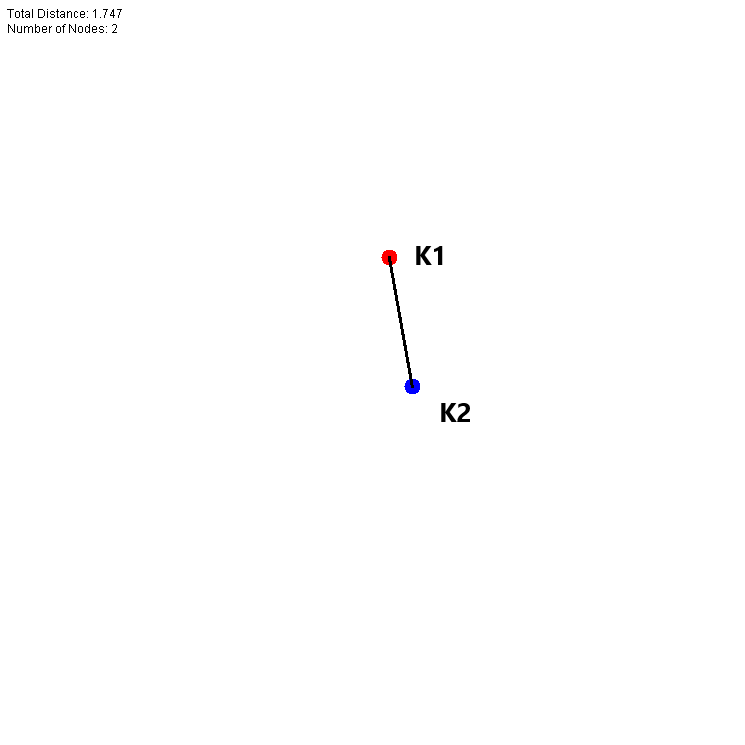
\includegraphics[width=0.6\textwidth]{./Bilder/insertFirst/insert_first_BAD_ex_1.PNG}
        }
    \end{center}
    \phantomcaption
\end{figure}
\begin{figure}[H]\ContinuedFloat
    \begin{center}
        \subfloat[$m = 3$\label{app:subfig:insert-first-BAD-m3}]{%
        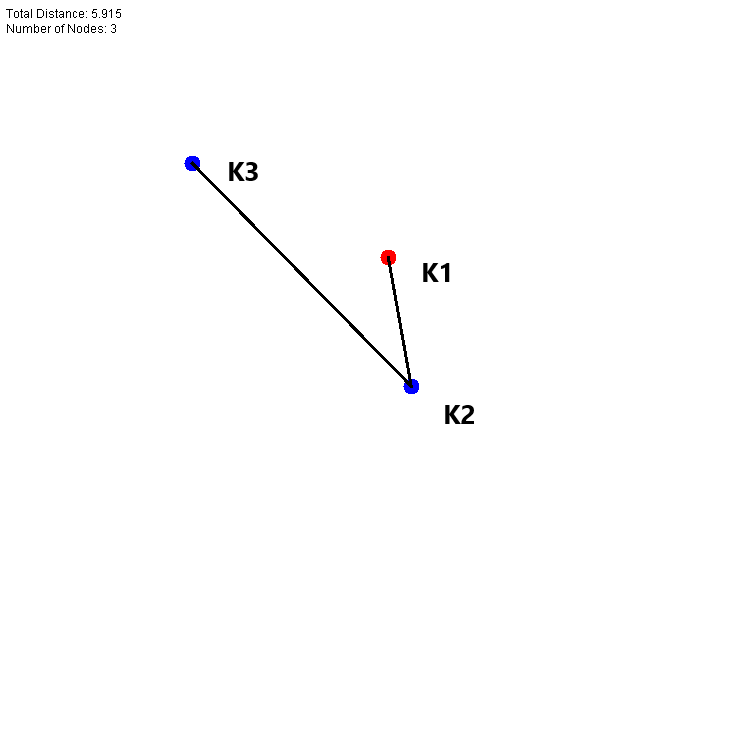
\includegraphics[width=0.6\textwidth]{./Bilder/insertFirst/insert_first_BAD_ex_2.PNG}
        }
    \end{center}
    \phantomcaption
\end{figure}
\begin{figure}[H]\ContinuedFloat
    \begin{center}
        \subfloat[$m = 4$\label{app:subfig:insert-first-BAD-m4}]{%
        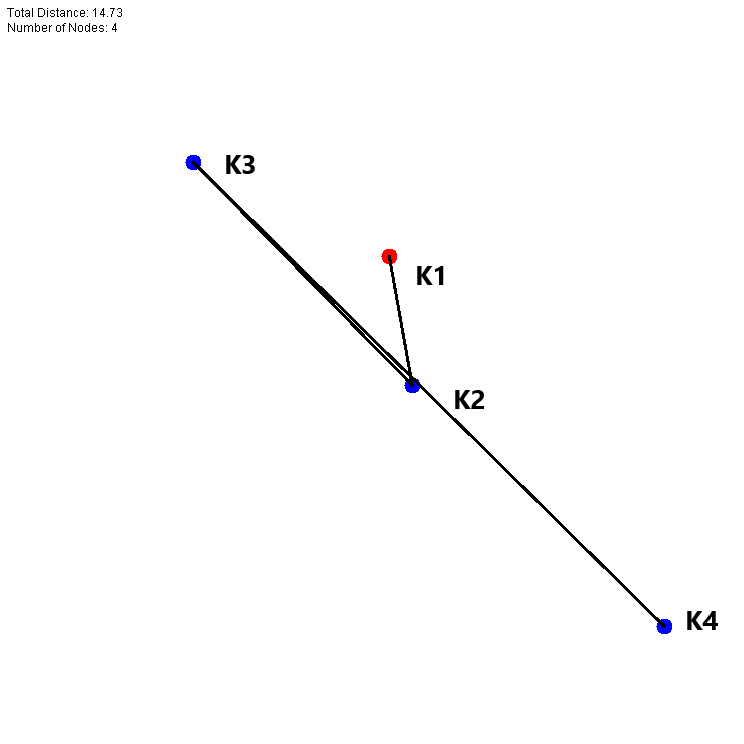
\includegraphics[width=0.6\textwidth]{./Bilder/insertFirst/insert_first_BAD_ex_3.PNG}
        }
    \end{center}
    \phantomcaption
\end{figure}
\begin{figure}[H]\ContinuedFloat
    \begin{center}
        \subfloat[$m = 5$\label{app:subfig:insert-first-BAD-m5}]{%
        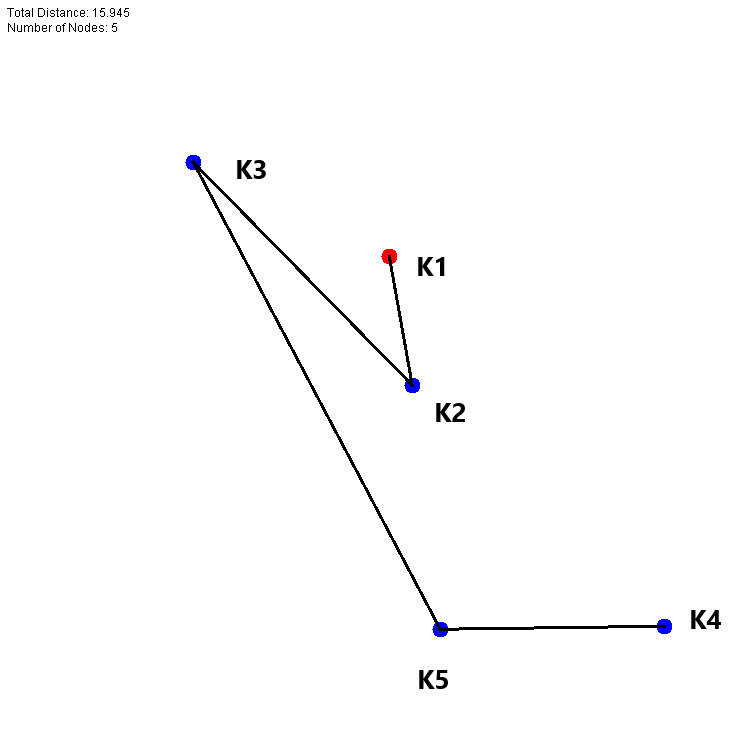
\includegraphics[width=0.6\textwidth]{./Bilder/insertFirst/insert_first_BAD_ex_4.PNG}
        }
    \end{center}
    \label{app:fig:insert-first-BAD-example-full}
    \caption{Insert-First: Schlechtes Beispiel}
\end{figure}


% INSERT FIRST GOOD EXAMPLE FULL
\begin{figure}[H]
    \begin{center}
        \subfloat[$m = 2$\label{app:subfig:insert-first-GOOD-m2}]{%
        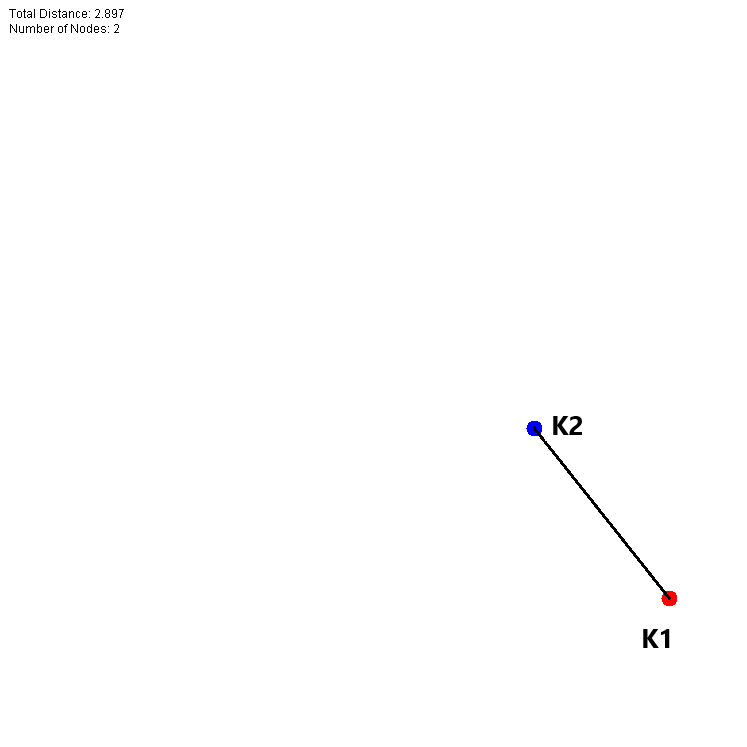
\includegraphics[width=0.6\textwidth]{./Bilder/insertFirst/insert_first_ex_1.PNG}
        }
    \end{center}
    \phantomcaption
\end{figure}
\begin{figure}[H]\ContinuedFloat
    \begin{center}
        \subfloat[$m = 3$\label{app:subfig:insert-first-GOOD-m3}]{%
        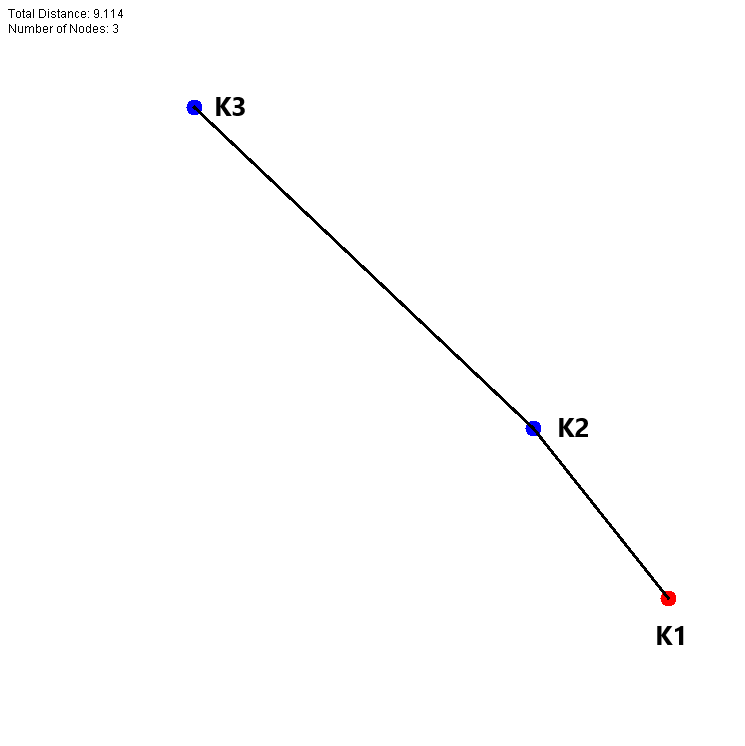
\includegraphics[width=0.6\textwidth]{./Bilder/insertFirst/insert_first_ex_2.PNG}
        }
    \end{center}
    \phantomcaption
\end{figure}
\begin{figure}[H]\ContinuedFloat
    \begin{center}
        \subfloat[$m = 4$\label{app:subfig:insert-first-GOOD-m4}]{%
        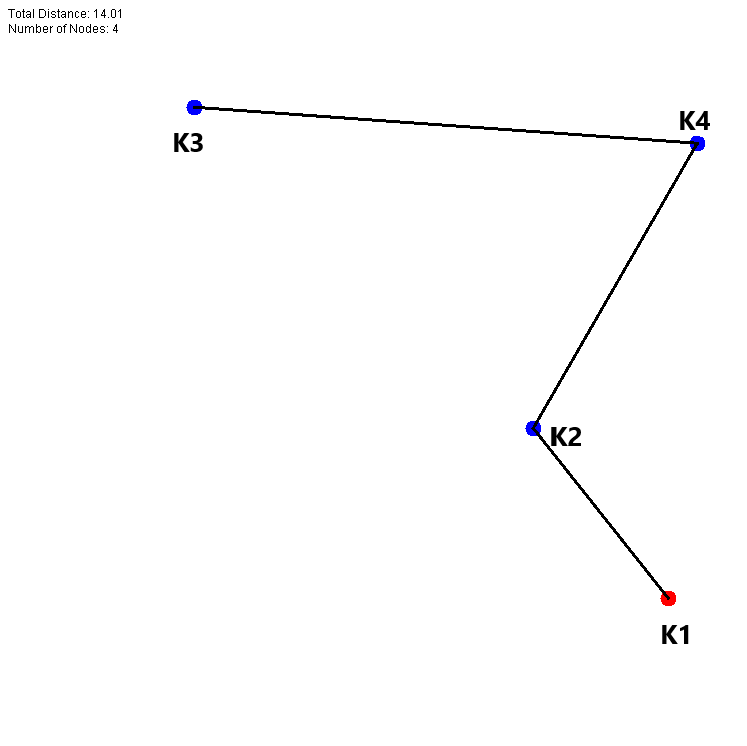
\includegraphics[width=0.6\textwidth]{./Bilder/insertFirst/insert_first_ex_3.PNG}
        }
    \end{center}
    \phantomcaption
\end{figure}
\begin{figure}[H]\ContinuedFloat
    \begin{center}
        \subfloat[$m = 5$\label{app:subfig:insert-first-GOOD-m5}]{%
        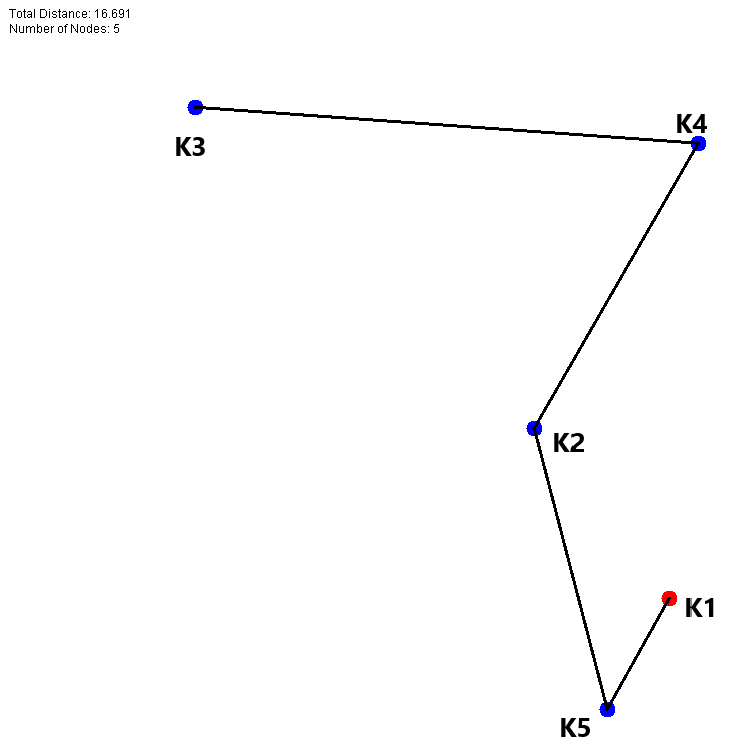
\includegraphics[width=0.6\textwidth]{./Bilder/insertFirst/insert_first_ex_4.PNG}
        }
    \end{center}
    \caption{Insert-First: Gutes Beispiel}
    \label{app:fig:insert-first-GOOD-example-full}
\end{figure}

% INSERT FURTHEST BAD EXAMPLE FULL
\begin{figure}[H]
    \begin{center}
        \subfloat[$m = 1$\label{app:subfig:insert-furthest-BAD-m1}]{%
        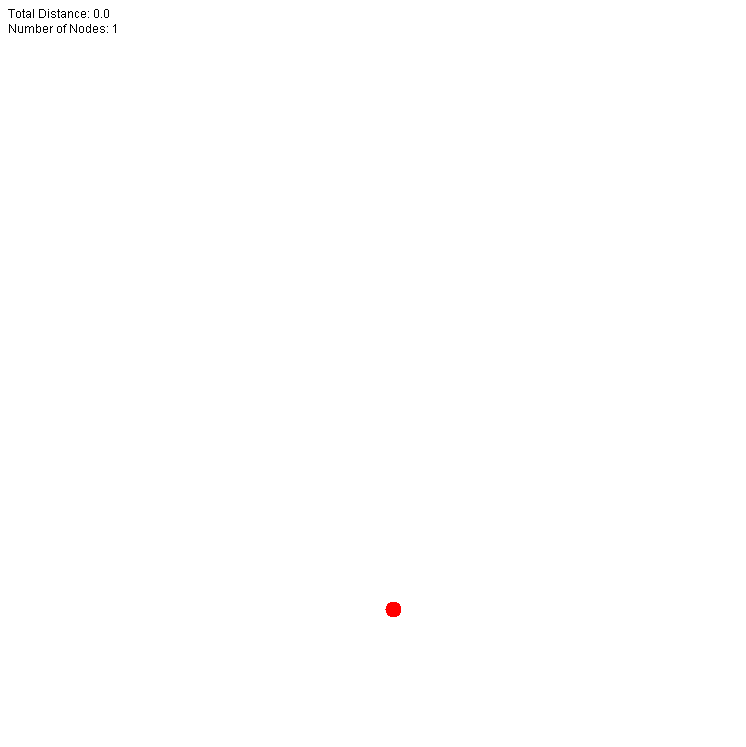
\includegraphics[width=0.6\textwidth]{./Bilder/insertFurthest/insert_furthest_ex_BAD_1.PNG}
        }
    \end{center}
    \phantomcaption
\end{figure}
\begin{figure}[H]\ContinuedFloat
    \begin{center}
        \subfloat[$m = 2$\label{app:subfig:insert-furthest-BAD-m2}]{%
        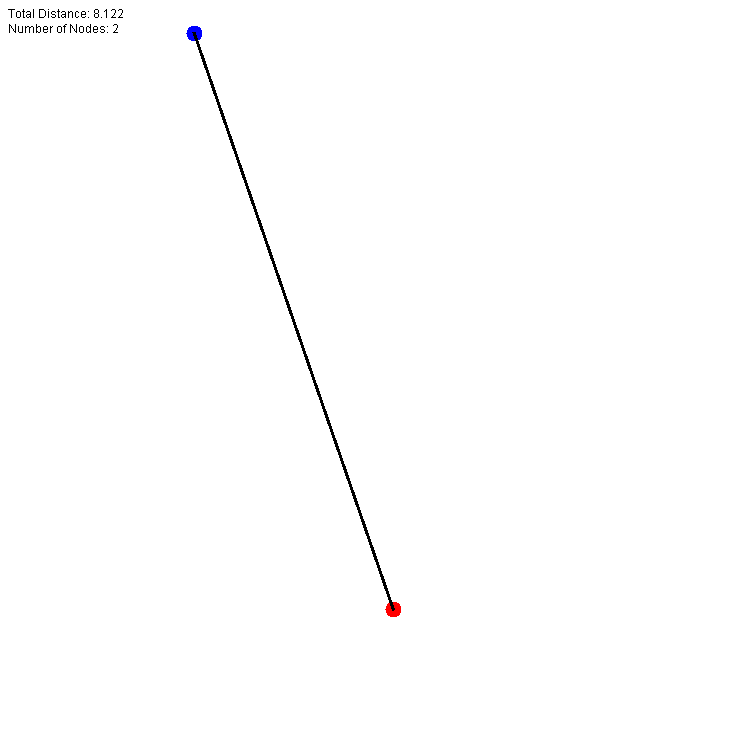
\includegraphics[width=0.6\textwidth]{./Bilder/insertFurthest/insert_furthest_ex_BAD_2.PNG}
        }
    \end{center}
    \phantomcaption
\end{figure}
\begin{figure}[H]\ContinuedFloat
    \begin{center}
        \subfloat[$m = 3$\label{app:subfig:insert-furthest-BAD-m3}]{%
        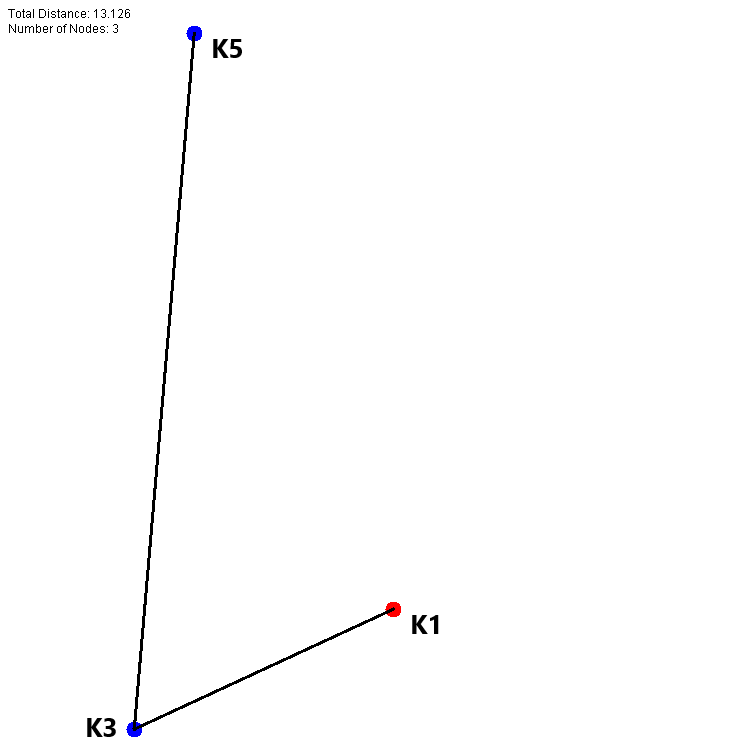
\includegraphics[width=0.6\textwidth]{./Bilder/insertFurthest/insert_furthest_ex_BAD_3.PNG}
        }
    \end{center}
    \phantomcaption
\end{figure}
\begin{figure}[H]\ContinuedFloat
    \begin{center}
        \subfloat[$m = 4$\label{app:subfig:insert-furthest-BAD-m4}]{%
        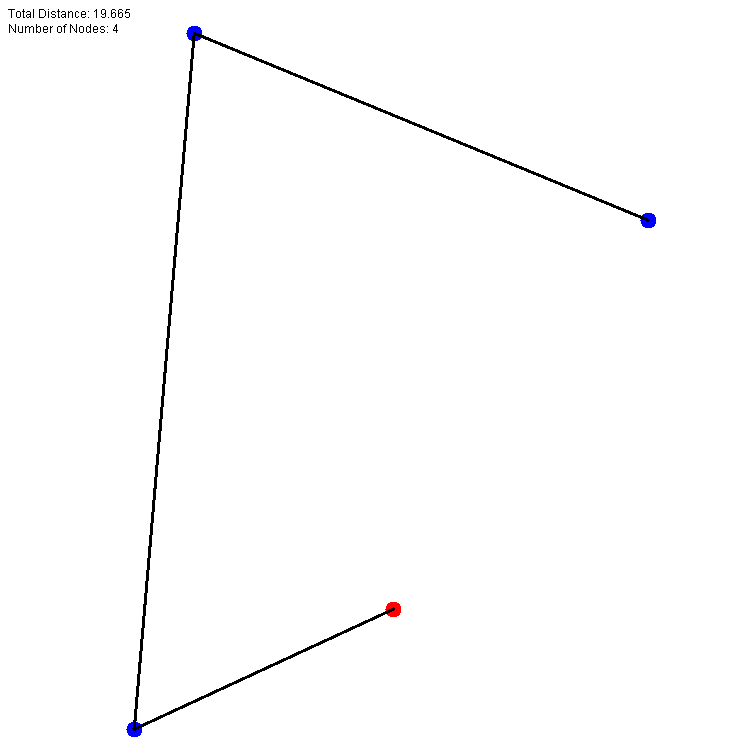
\includegraphics[width=0.6\textwidth]{./Bilder/insertFurthest/insert_furthest_ex_BAD_4.PNG}
        }
    \end{center}
    \phantomcaption
\end{figure}
\begin{figure}[H]\ContinuedFloat
    \begin{center}
        \subfloat[$m = 5$\label{app:subfig:insert-furthest-BAD-m5}]{%
        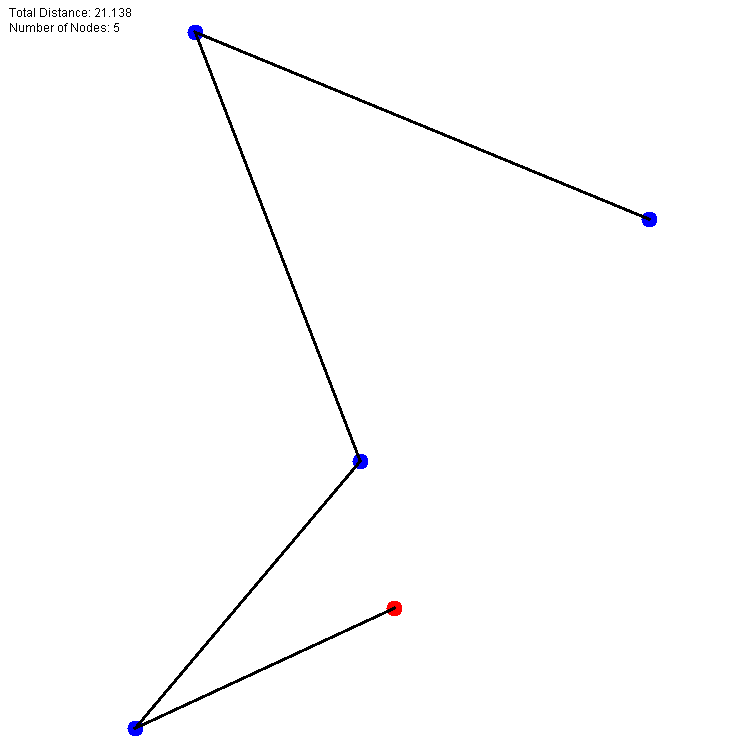
\includegraphics[width=0.6\textwidth]{./Bilder/insertFurthest/insert_furthest_ex_BAD_5.PNG}
        }
    \end{center}
    \caption{Insert-Furthest: Schlechtes Beispiel}
    \label{app:fig:insert-furthest-BAD-example-full}
\end{figure}

% INSERT FURTHEST GOOD EXAMPLE FULL
\begin{figure}[H]
    \begin{center}
        \subfloat[$m = 1$\label{app:subfig:insert-furthest-GOOD-m1}]{%
        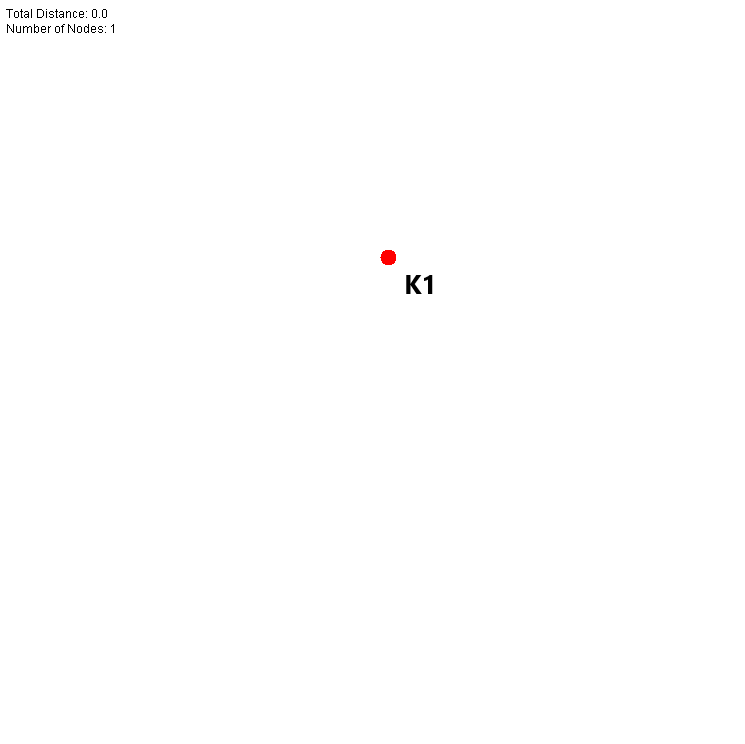
\includegraphics[width=0.6\textwidth]{./Bilder/insertFurthest/insert_furthest_ex_1.PNG}
        }
    \end{center}
    \phantomcaption
\end{figure}
\begin{figure}[H]\ContinuedFloat
    \begin{center}
        \subfloat[$m = 2$\label{app:subfig:insert-furthest-GOOD-m2}]{%
        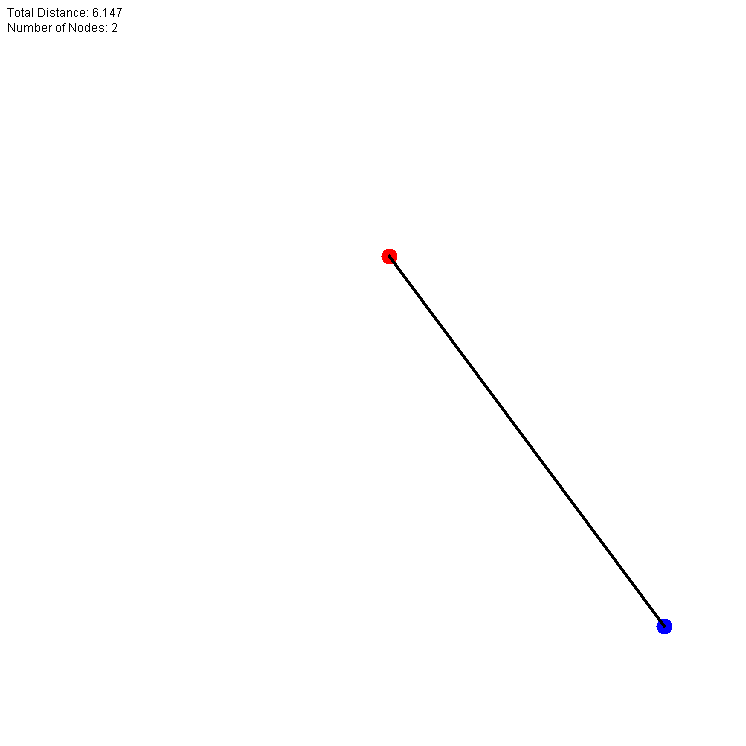
\includegraphics[width=0.6\textwidth]{./Bilder/insertFurthest/insert_furthest_ex_2.PNG}
        }
    \end{center}
    \phantomcaption
\end{figure}
\begin{figure}[H]\ContinuedFloat
    \begin{center}
        \subfloat[$m = 3$\label{app:subfig:insert-furthest-GOOD-m3}]{%
        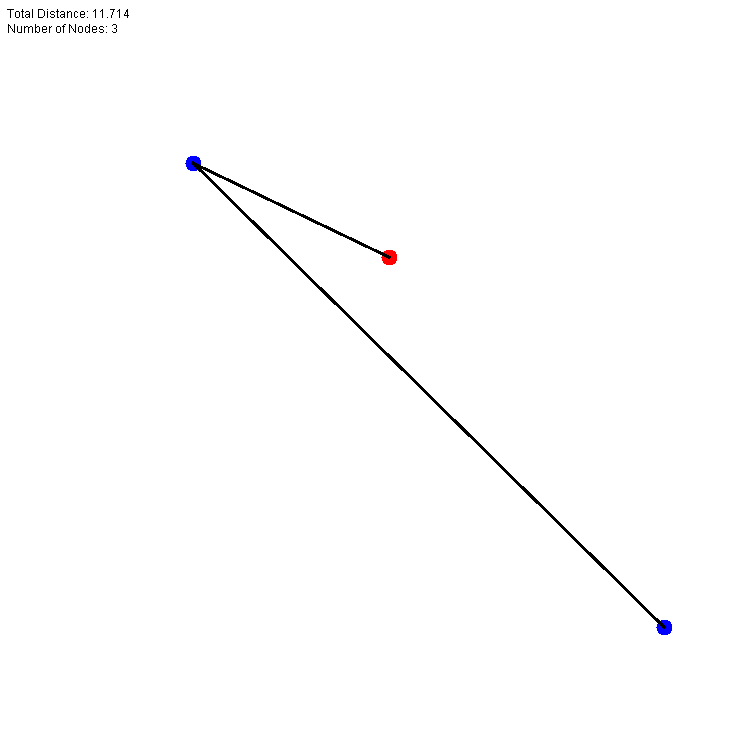
\includegraphics[width=0.6\textwidth]{./Bilder/insertFurthest/insert_furthest_ex_3.PNG}
        }
    \end{center}
    \phantomcaption
\end{figure}
\begin{figure}[H]\ContinuedFloat
    \begin{center}
        \subfloat[$m = 4$\label{app:subfig:insert-furthest-GOOD-m4}]{%
        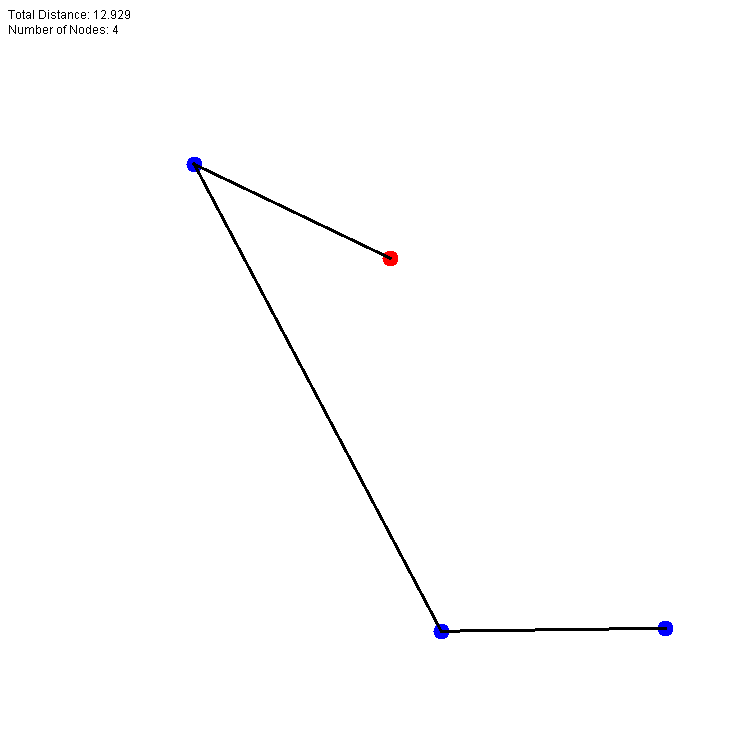
\includegraphics[width=0.6\textwidth]{./Bilder/insertFurthest/insert_furthest_ex_4.PNG}
        }
    \end{center}
    \phantomcaption
\end{figure}
\begin{figure}[H]\ContinuedFloat
    \begin{center}
        \subfloat[$m = 5$\label{app:subfig:insert-furthest-BAD-m5}]{%
        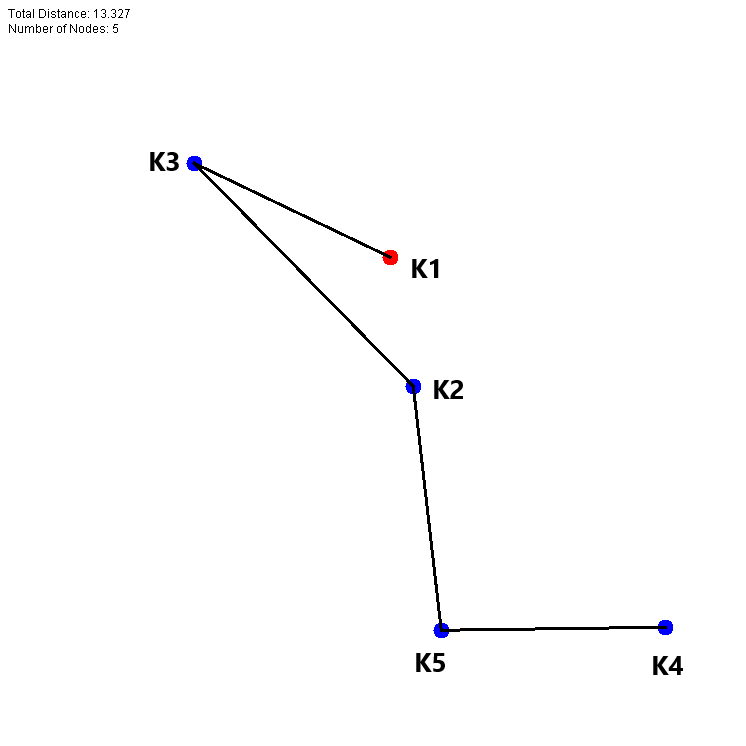
\includegraphics[width=0.6\textwidth]{./Bilder/insertFurthest/insert_furthest_ex_5.PNG}
        }
    \end{center}
    \caption{Insert-Furthest: Gutes Beispiel}
    \label{app:fig:insert-furthest-GOOD-example-full}
\end{figure}

% INSERT CLOSEST BAD EXAMPLE FULL
\begin{figure}[H]
    \begin{center}
        \subfloat[$m = 2$\label{app:subfig:insert-closest-BAD-m1}]{%
        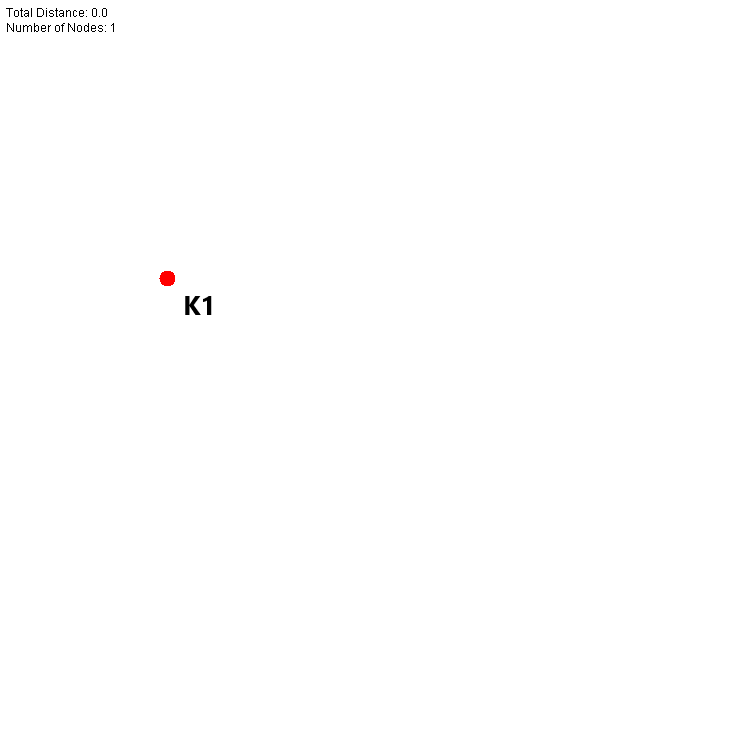
\includegraphics[width=0.6\textwidth]{./Bilder/insertClosest/insert_closest_ex_BAD_1.PNG}
        }
    \end{center}
    \phantomcaption
\end{figure}
\begin{figure}[H]\ContinuedFloat
    \begin{center}
        \subfloat[$m = 2$\label{app:subfig:insert-closest-BAD-m2}]{%
        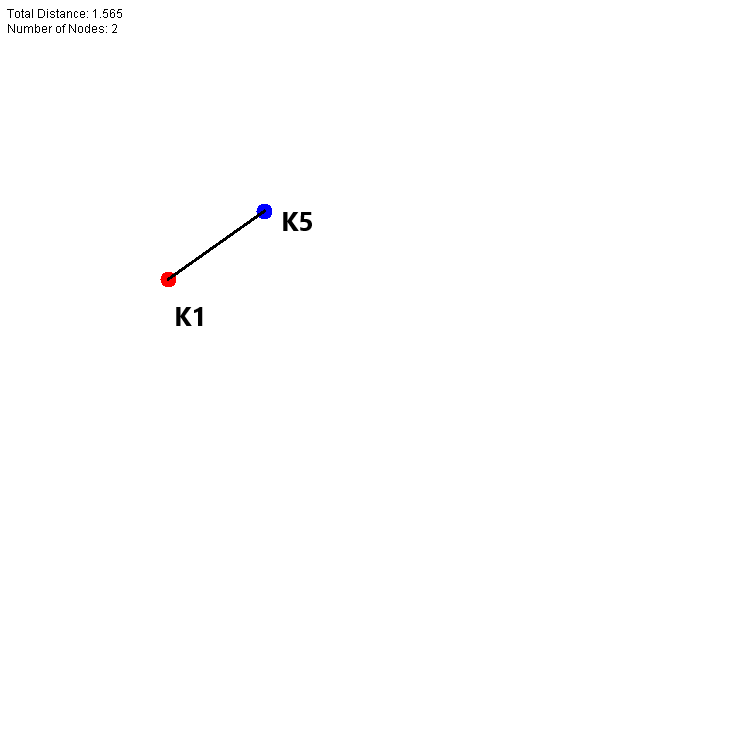
\includegraphics[width=0.6\textwidth]{./Bilder/insertClosest/insert_closest_ex_BAD_2.PNG}
        }
    \end{center}
    \phantomcaption
\end{figure}
\begin{figure}[H]\ContinuedFloat
    \begin{center}
        \subfloat[$m = 3$\label{app:subfig:insert-closest-BAD-m3}]{%
        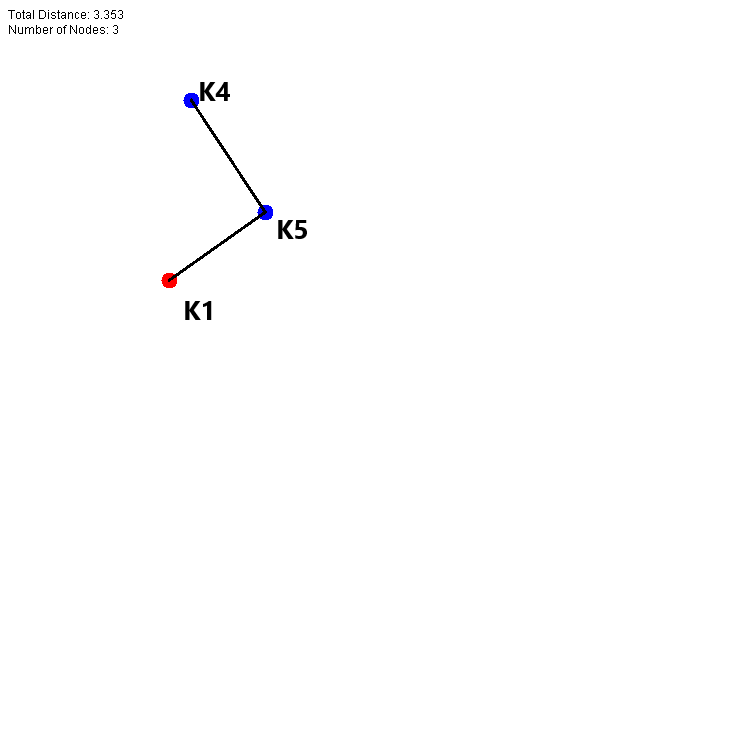
\includegraphics[width=0.6\textwidth]{./Bilder/insertClosest/insert_closest_ex_BAD_3.PNG}
        }
    \end{center}
    \phantomcaption

\end{figure}
\begin{figure}[H]\ContinuedFloat
    \begin{center}
        \subfloat[$m = 4$\label{app:subfig:insert-closest-BAD-m4}]{%
        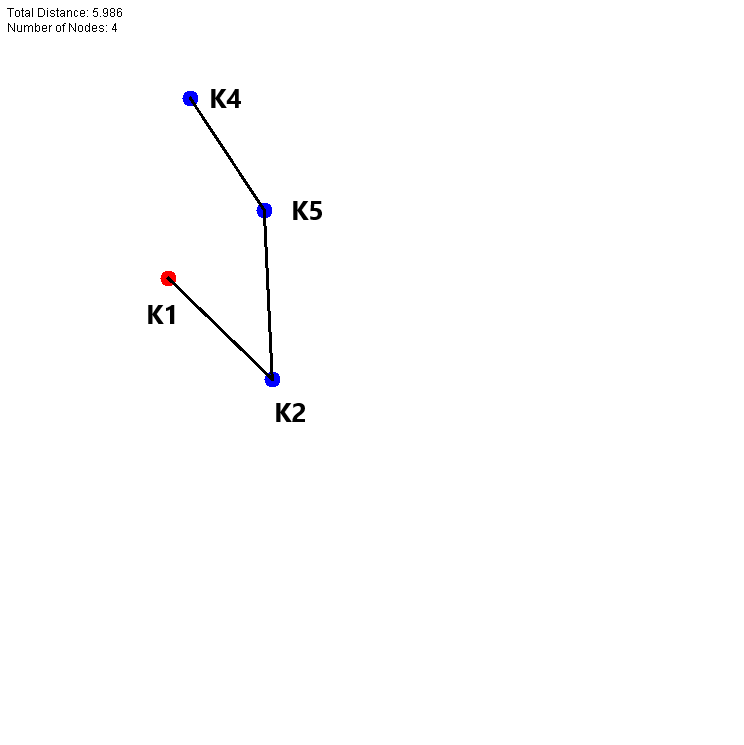
\includegraphics[width=0.6\textwidth]{./Bilder/insertClosest/insert_closest_ex_BAD_4.PNG}
        }
    \end{center}
    \phantomcaption

\end{figure}
\begin{figure}[H]\ContinuedFloat
    \begin{center}
        \subfloat[$m = 5$\label{app:subfig:insert-closest-BAD-m5}]{%
        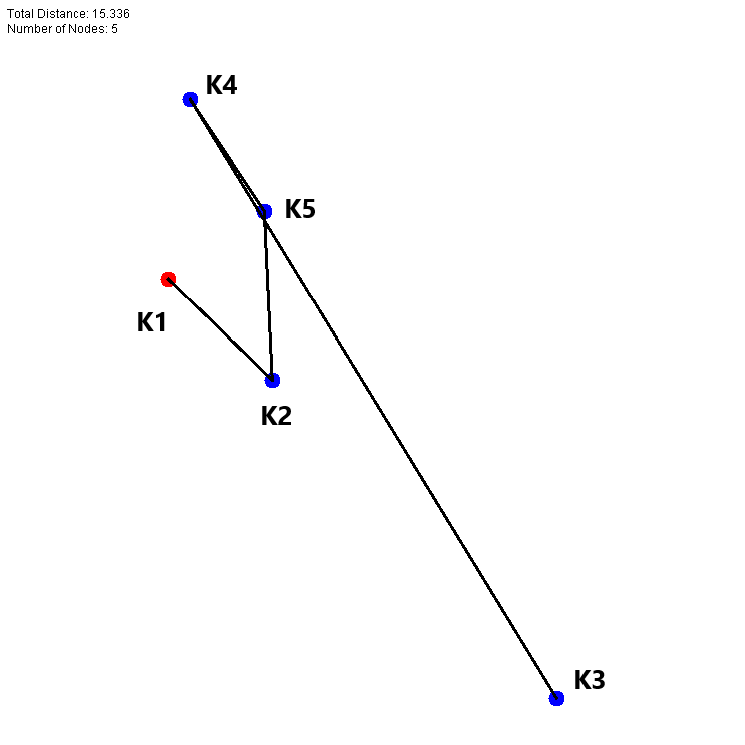
\includegraphics[width=0.55\textwidth]{./Bilder/insertClosest/insert_closest_ex_BAD_5.PNG}
        }
    \end{center}
    \caption{Insert-Closest: Schlechtes Beispiel}
    \label{app:fig:insert-closest-BAD-example-full}
\end{figure}

% INSERT CLOSEST GOOD EXAMPLE ??

\begin{figure}[H]
    \begin{center}
        \subfloat[Pfad mit einem Crossover\label{app:subfig:40-nodes-with-crossover}]{%
        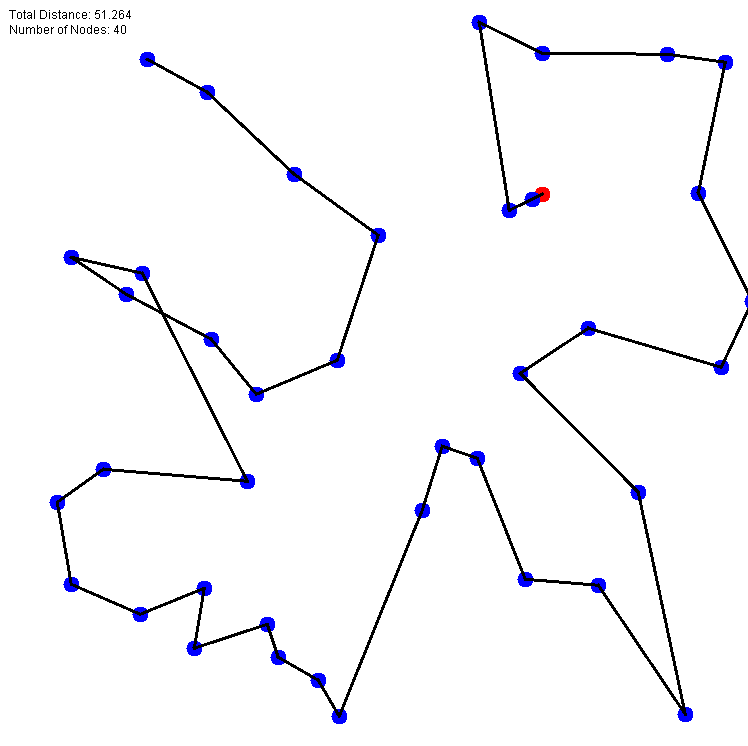
\includegraphics[width=0.55\textwidth]{./Bilder/crossover/40_nodes_with_crossover}
        }
    \end{center}
    \phantomcaption

\end{figure}
\begin{figure}[H]
    \begin{center}
        \subfloat[Pfad mit aufgelöstem Crossover\label{app:subfig:40-nodes-without-crossover}]{%
        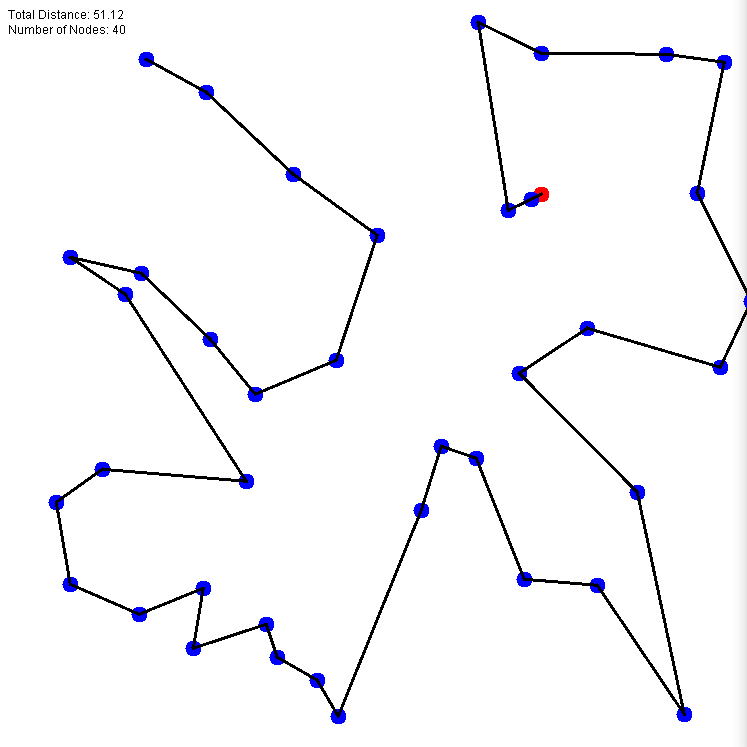
\includegraphics[width=0.55\textwidth]{./Bilder/crossover/40_nodes_without_crossover.PNG}
        }
    \end{center}
    \caption{Pfad aus 40 Knoten mit und ohne Crossover}
    \label{app:fig:40-nodes-crossover-example}
\end{figure}

\begin{figure}[H]
    \begin{center}
        \subfloat[Teilpfad vor Nachbesserung\label{app:subfig:40-nodes-before-after-control}]{
            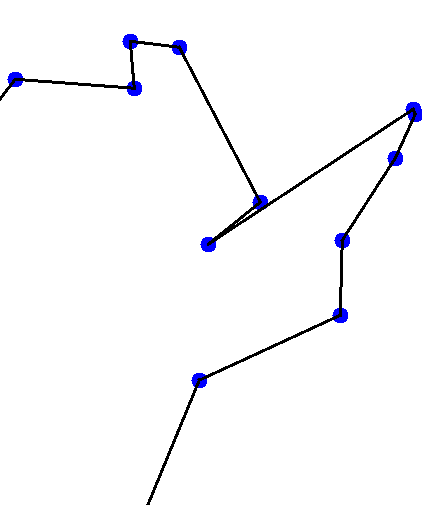
\includegraphics[width=0.3\textwidth]{Bilder/afterControl/before_after_control.PNG}
        }
    \end{center}
    \phantomcaption

\end{figure}

\begin{figure}[H]
    \begin{center}
        \subfloat[Teilpfad nach Nachbesserung\label{app:subfig:40-nodes-after-after-control}]{
            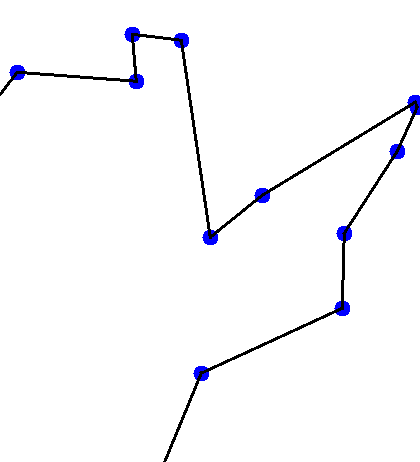
\includegraphics[width=0.3\textwidth]{Bilder/afterControl/after_after_control.PNG}
        }
    \end{center}
    \caption{Beispiel für eine Nachbesserung, Teilpfad}
\end{figure}

\section{Algorithmen}
\begin{algorithm}
    \caption{Einfügen eines neuen Knoten in einen Pfad}
    \label{alg:merge-node-into-path}
    \begin{algorithmic}[1]
        \Require Pfad $P = p_1,\ldots,p_n$ mit $\forall p \in G$
        \Comment Jedes p ist Knoten in Graph $G$
        \Require Knoten $K^*$, Index $i$, $i \leq n + 1$
        \Comment neuer Knoten $K^*$, einzufügen an Index $i$
        \For{$a \gets n$, $a \geq i$, $a \gets a+1$}
            \State $p_{a+1} \gets p_a$
        \EndFor
        \State $p_i \gets K^*$ \\
        \Return $P$
    \end{algorithmic}
\end{algorithm}


\begin{algorithm}
    \caption{Tauschen von Knoten auf einem Graph zwischen zwei eingegebenen Knoten}\label{alg:test-alg}
    \begin{algorithmic}[1]
        \Require Graph $G$, Knotenpaare $A_1,A_2$ und $B_1,B_2$
        \Require $G=k_1,k_2,\cdots,k_n$, $n>4$
        \State $i_{A_2} \gets$ \textsc{index}($A_2$)
        \State $i_{B_1} \gets$ \textsc{index}($B_1$)
        \If{$i_{A_2} > i_{B_1}$}
            \State \textsc{swap}($i_{A_2}$, $i_{B_1}$) 
            \Comment \textsc{swap} weißt beiden Parametern den Wert des anderen zu
        \EndIf
        \While{$i_{A_2} < i_{B_1}$}
            \State \textsc{swap}($k_{i_{A_2}}$,$k_{i_{B_1}}$)
        \EndWhile
    \end{algorithmic}
\end{algorithm}

\begin{algorithm}
    \caption{Berechnung der Distanz zwischen zwei Knoten}
    \label{alg:calc-distance-two-nodes}
    \begin{algorithmic}[1]
        \Require Knoten $A$, Knoten $B$
        % \Require $P=p_1,\cdots,\p_n$, $n \geq 2$
        \State $d \gets \sqrt{|x_A - x_B|^2 + |y_A - y_B|^2}$\\
        \Return $d$
        % \State 
    \end{algorithmic}
\end{algorithm}

\begin{algorithm}
    \caption{Berechnung der Gesamtdistanz eines Pfads}
    \label{alg:calc-total-distance}
    \begin{algorithmic}[1]
        \Require Pfad $P$
        \Require $P=p_1,\cdots,p_n$, $n \geq 2$
        \State sum $\gets 0$
        \For{$a \gets 2$, $a \leq n$, $a \gets a + 1$}
            \State sum $\gets sum + \textrm{\textsc{distance}}(p_{a-1}, p_a)$
        \EndFor\\
        \Return sum
        % \State 
    \end{algorithmic}
\end{algorithm}

\begin{algorithm}
    \caption{Erkennen von Überkreuzungen}
    \label{alg:check-point-in-rect}
    \begin{algorithmic}[1]
        \Require Knoten $A_1,A_2$, Punkt $P$
        \State score $\gets 0$
        \If{$x_{A_1} > x_{A_2}$}
            \If{$x_P > x_{A_2}$ \textbf{and} $x_P < x_{A_1}$}
                \State score $\gets$ score $+ 1$
            \EndIf
        \Else
            \If{$x_P < x_{A_2}$ \textbf{and} $x_P > x_{A_1}$}
                \State score $\gets$ score $+ 1$
            \EndIf
        \EndIf

        \If{$y_{A_1} > y_{A_2}$}
            \If{$y_P < y_{A_1}$ \textbf{and} $y_P > y_{A_2}$}
                \State score $\gets$ score $+ 1$
            \EndIf
        \Else
            \If{$y_P > y_{A_1}$ \textbf{and} $y_P < y_{A_2}$}
                \State score $\gets$ score $+ 1$
            \EndIf
        \EndIf\\
        \Return (score $== 2$)
        \Comment score $==2$ gibt wahr zurück und signalisiert, dass $P$ im Rechteck von $A_1$ und $A_2$ ist
    \end{algorithmic}
\end{algorithm}

\begin{algorithm}
    \caption{Tauschen von Knoten auf einem Graph zwischen zwei eingegebenen Knoten}
    \label{alg:swap-nodes-inbetween}
    \begin{algorithmic}[1]
        \Require Graph $G$, Knotenpaare $A_1,A_2$ und $B_1,B_2$
        \Require $G=k_1,k_2,\cdots,k_n$, $n>4$
        \State $i_{A_2} \gets$ \textsc{index}($A_2$)
        \State $i_{B_1} \gets$ \textsc{index}($B_1$)
        \If{$i_{A_2} > i_{B_1}$}
            \State \textsc{swap}($i_{A_2}$, $i_{B_1}$) 
            \Comment \textsc{swap} weißt beiden Parametern den Wert des anderen zu
        \EndIf
        \While{$i_{A_2} < i_{B_1}$}
            \State \textsc{swap}($k_{i_{A_2}}$,$k_{i_{B_1}}$)
        \EndWhile
    \end{algorithmic}
\end{algorithm}